\chapter{Mod�le du syst�me}
          * Cas d'utilisation (diagrammes UML)
          * Mod�le abstrait de donn�es (diagrammes UML) 


\begin{figure}[h!t]
  \centering
  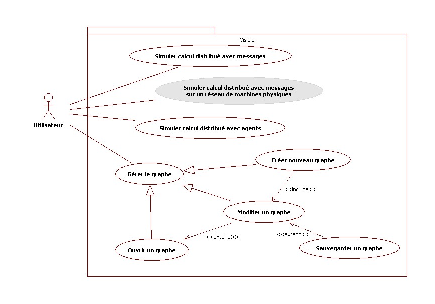
\includegraphics[width=14cm]{img/visidia_cu_vue_generale}
  \caption{Cas d'utilisation : Vue g�n�rale de \visidia} 
  \label{fig:cu_vue_generale}
\end{figure}


\begin{figure}[h!t]
  \centering
  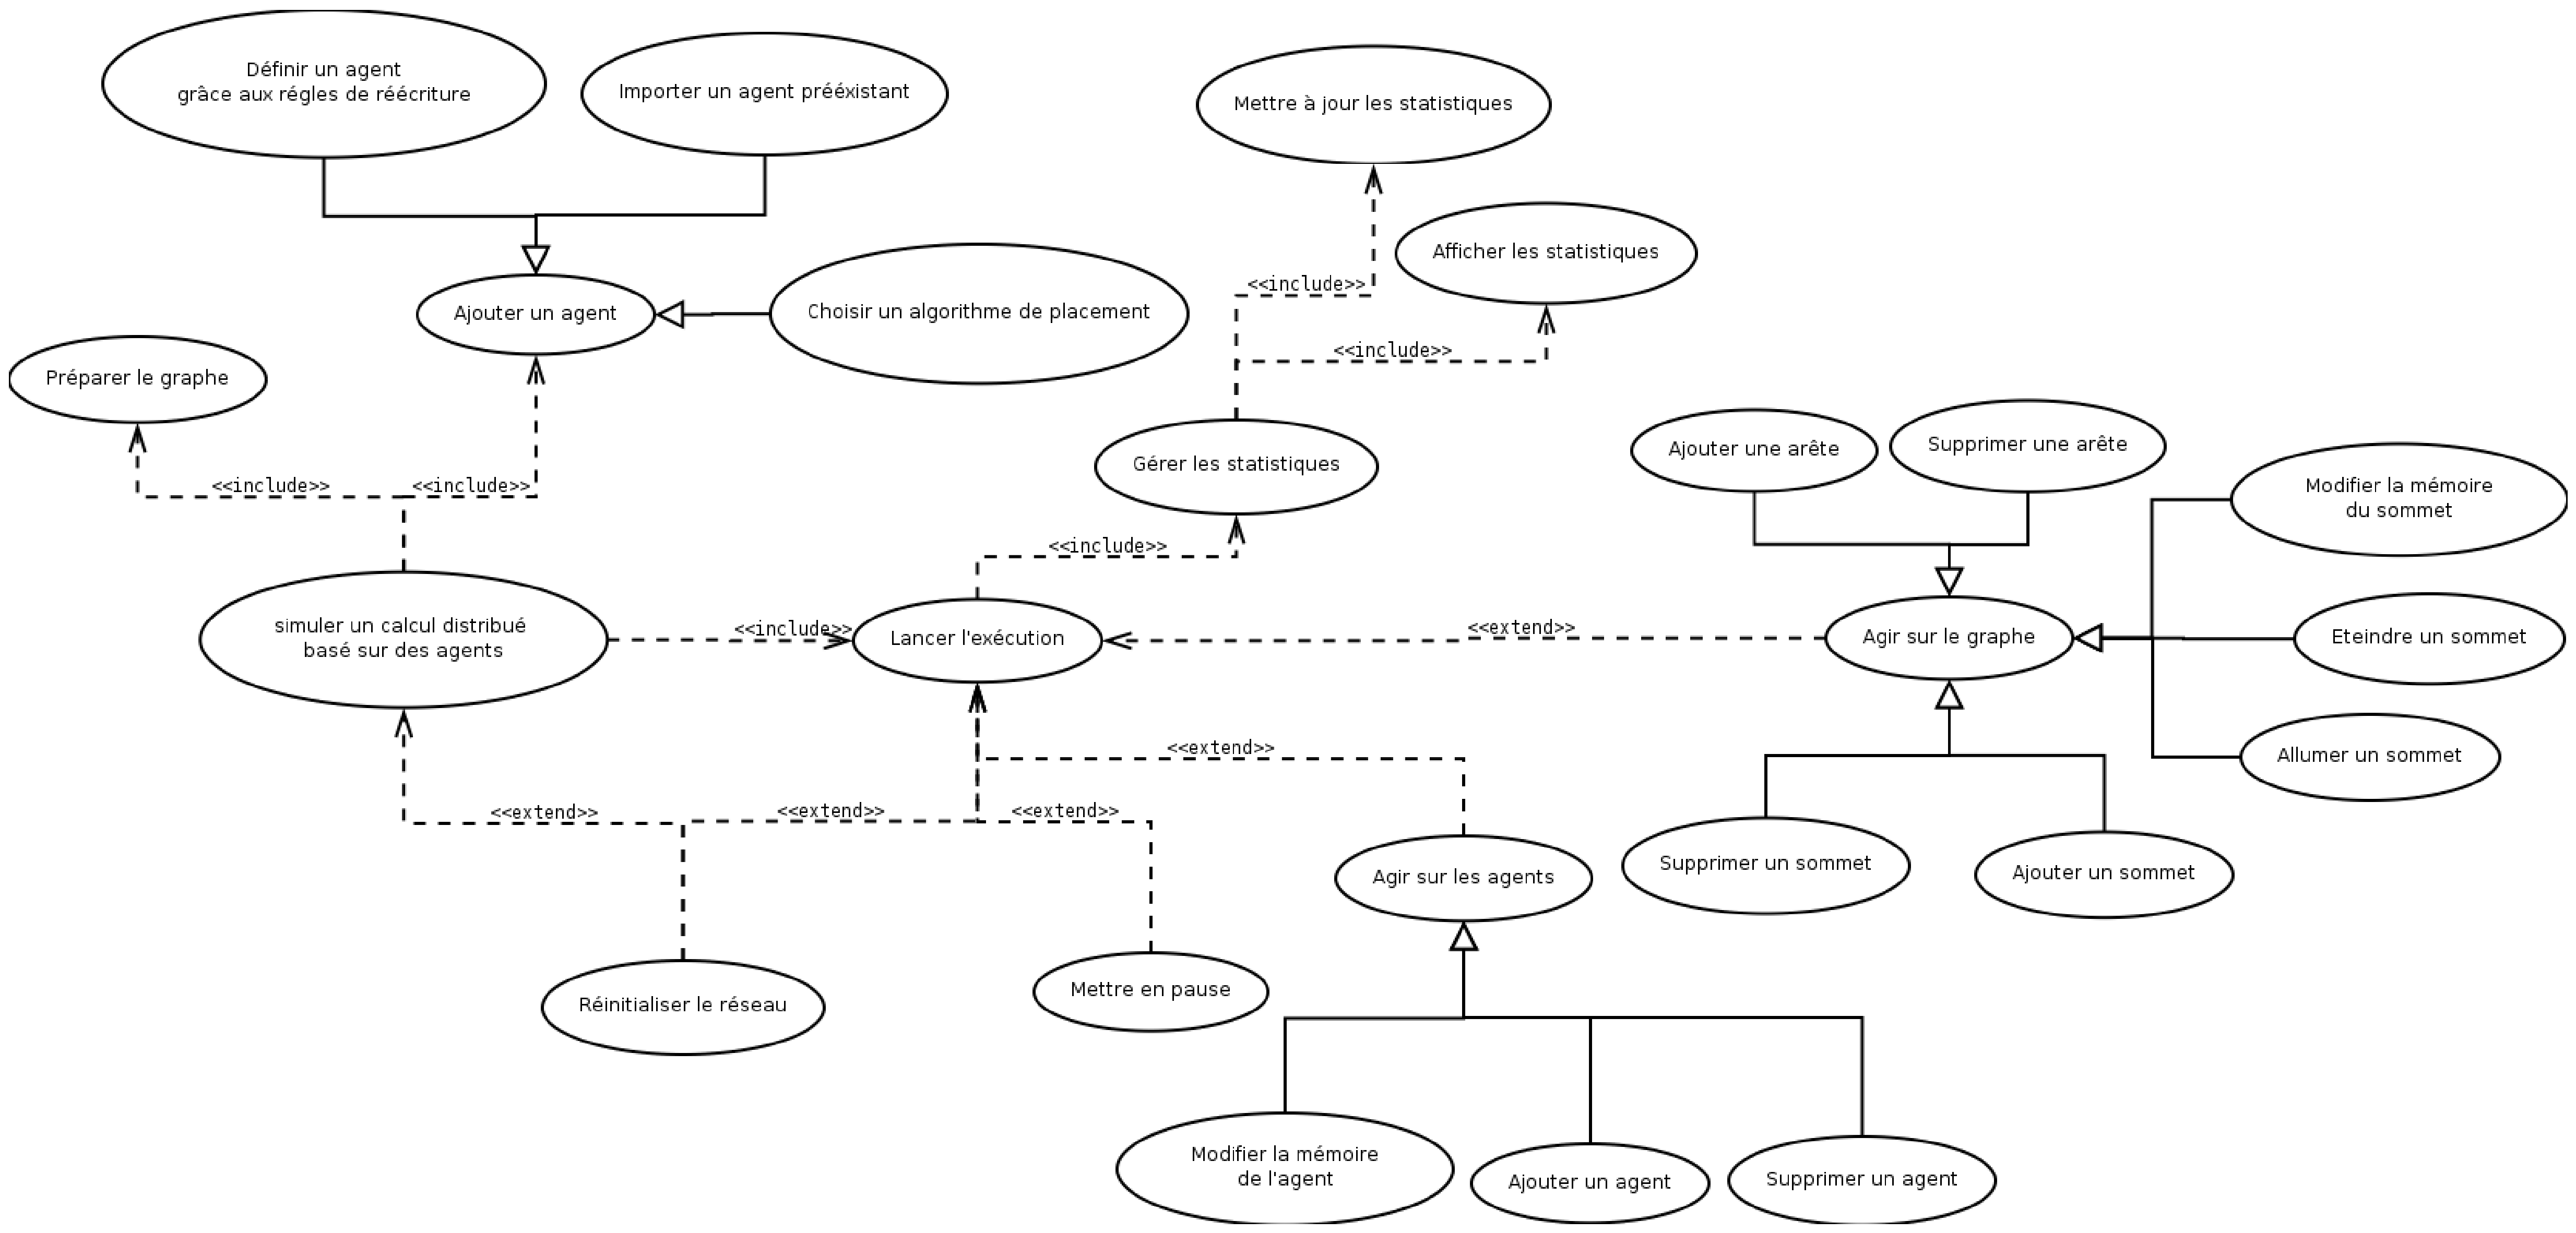
\includegraphics[width=24cm,angle=90]{img/visidia_cu_simuler_agent}
  \caption{Cas d'utilisation : Simuler agent} 
  \label{fig:cu_simuler}
\end{figure}


%\begin{figure}[h!t]
%  \centering
%  
\includegraphics[width=14cm]{img/visidia_cu_agir_agent}
%  \caption{Cas d'utilisation : Vue g�n�rale de \visidia} 
%  \label{fig:cu_vue_generale}
%\end{figure}


%\begin{figure}[h!t]
%  \centering
%  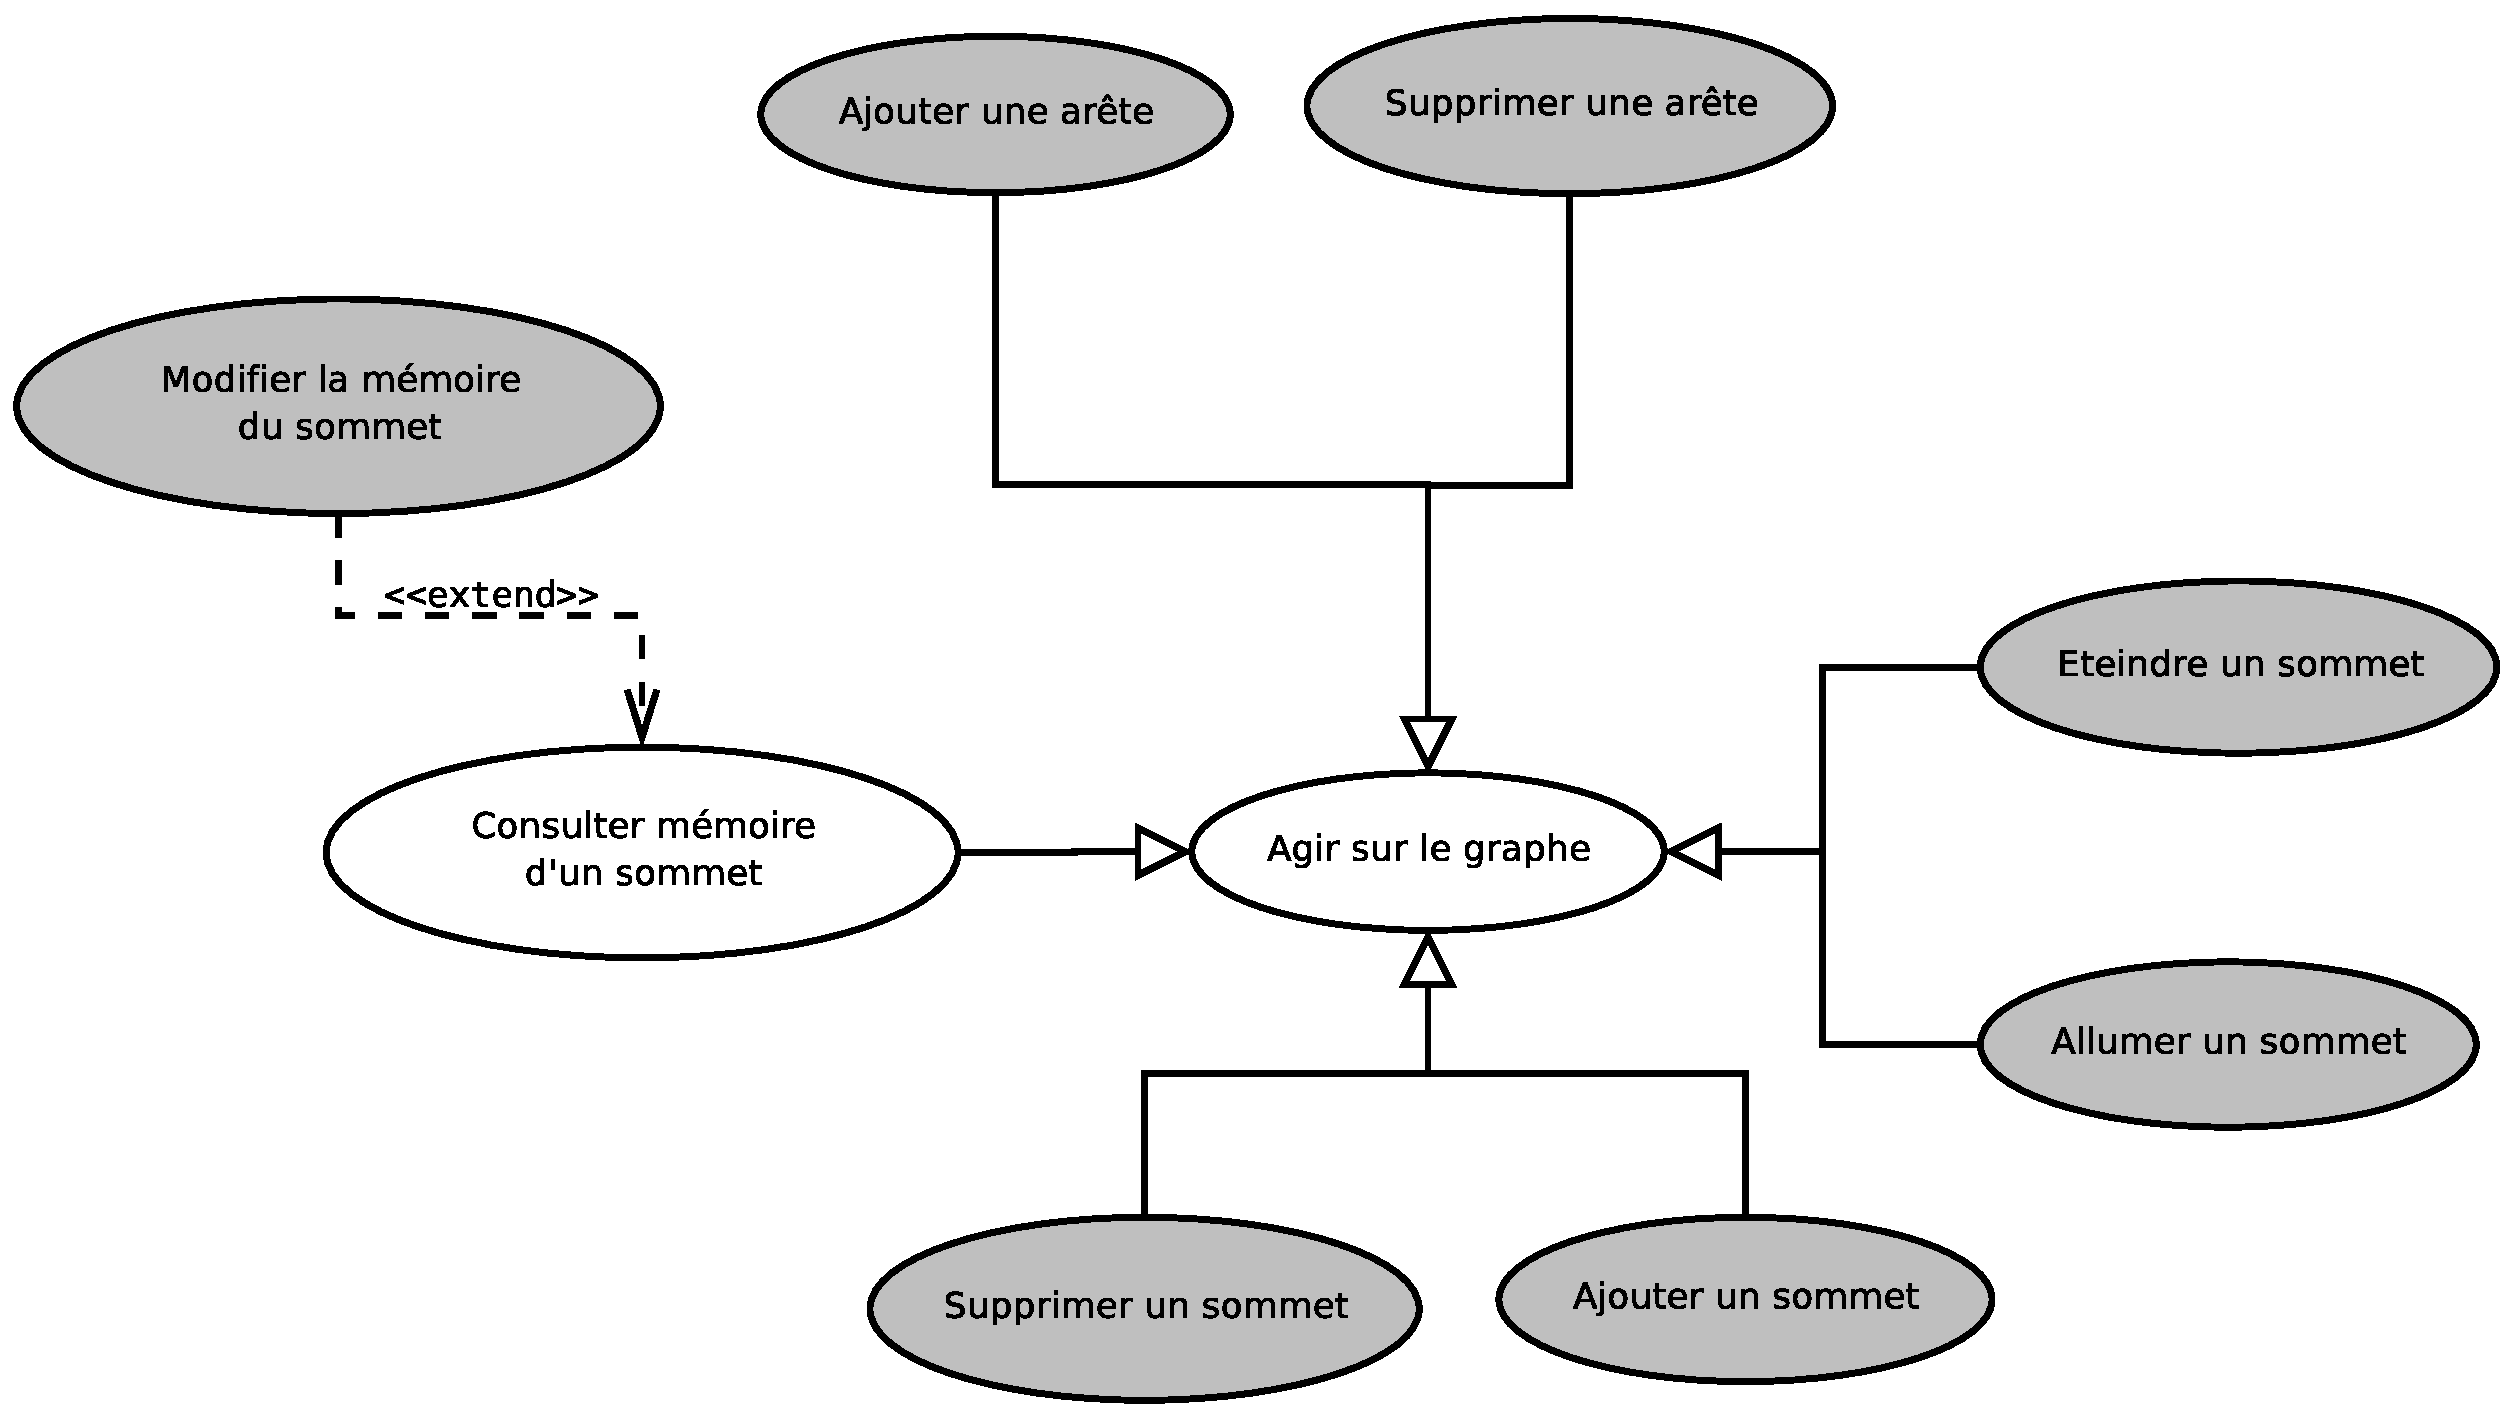
\includegraphics[width=14cm]{img/visidia_cu_agir_graphe}
%  \caption{Cas d'utilisation : Vue g�n�rale de \visidia} 
%  \label{fig:cu_vue_generale}
%\end{figure}


%\begin{figure}[h!t]
%  \centering
%  
\includegraphics[width=14cm]{img/visidia_cu_ajouter_agent}
%  \caption{Cas d'utilisation : Vue g�n�rale de \visidia} 
%  \label{fig:cu_vue_generale}
%\end{figure}

